 \documentclass [12pt]{article} 

\usepackage {amsmath}
\usepackage {amsthm}
\usepackage {amssymb}
\usepackage {graphicx} 
\usepackage {float}
\usepackage {multirow}
\usepackage {xcolor}
\usepackage [ruled,vlined,commentsnumbered,titlenotnumbered]{algorithm2e} \usepackage {array} 
\usepackage {booktabs} 
\usepackage {url} 
\usepackage {parskip} 
\usepackage [margin=1in]{geometry} 
\usepackage [T1]{fontenc} 
\usepackage {cmbright} 
\usepackage [many]{tcolorbox} 
\usepackage [colorlinks = true,
            linkcolor = blue,
            urlcolor  = blue,
            citecolor = blue,
            anchorcolor = blue]{hyperref} 
\usepackage {enumitem} 
\usepackage {xparse} 
\usepackage {verbatim}
\usepackage{algpseudocode}
\usepackage{listings}
\usepackage{xcolor}
\lstset { %
    language=C++,
    backgroundcolor=\color{black!5}, % set backgroundcolor
    basicstyle=\footnotesize,% basic font setting
}
\newtheorem{theorem}{Theorem}
\newtheorem{remark}{Remark}
\newtheorem{lemma}[theorem]{Lemma}
\theoremstyle{definition}
\newtheorem{definition}{Definition}[section]
\newtheorem{claim}{Claim}
\newtheorem{proposition}{Proposition}






\DeclareTColorBox {Solution}{}{breakable, title={Solution}} \DeclareTColorBox {Solution*}{}{breakable, title={Solution (provided)}} \DeclareTColorBox {Instruction}{}{boxrule=0pt, boxsep=0pt, left=0.5em, right=0.5em, top=0.5em, bottom=0.5em, arc=0pt, toprule=1pt, bottomrule=1pt} \DeclareDocumentCommand {\Expecting }{+m}{\textbf {[We are expecting:} #1\textbf {]}} \DeclareDocumentCommand {\Points }{m}{\textbf {(#1 pt.)}} 

\begin {document} 

\vspace {1em} 
\begin {Instruction} 
Adapted From Virginia Williams'lecture notes.
\end {Instruction}  

{\LARGE \textbf {COMP 285 (NC A\&T, Spr `22)}\hfill \textbf {Lecture 28} } 

\begin{centering}
\section*{More Greedy: Huffman Coding and MST}
\end{centering}


\section{Activity Selection}

Last lecture, we introduced the activity selection problem and walkted through a few possible candidates for greedy algorithms.

\begin{proposition}
For each $S_{i ,j}$, there is an optimal solution $A_{i ,j}$ containing $a_k \in S_{i ,j}$ of minimum finishing time $f_k$.
\end{proposition}
 

Note that if the proposition is true, when $f_k$ is minimum, then $A_{i ,k}$ is empty, as no activities can finish before $a_k$ ; thus, our optimal solution only depends on one other subproblem $A_{k ,j}$ (giving us a linear time algorithm). 


Here, we prove the proposition.

\begin{proof}

Let $a_k$ be the activity of minimum finishing time in $S_{i ,j}$. Let $A_{i ,j}$ be some maximum set of non-conflicting activities. Consider $A'_{i ,j} = A_{i ,j} \setminus {a_l} \cup {a_k}$ where $a_l$ is the activity of minimum finishing time in $A_{i ,j}$. It's clear that $|A'_{i ,j}| = |A_{i ,j}|$. We need to show that $A'_{i ,j}$ does not have conflicting activities. We know $a_l \in A_{i ,j} \subset S_{i ,j}$. This implies $f_l \geq f_k$ , since $a_k$ has the minimum finishing time in $S_{i ,j}$. 

All $a_t \in A_{i ,j} \setminus {a_l}$ don't conflict with $a_l $, which means that $s_t \geq f_l$ , which means that $s_t \geq f_k$ , so this means that no activity in $A_{i ,j} \setminus {a_l}$ can conflict with $a_k$ . Thus, $A'_{i ,j}$ is an optimal solution.
\end{proof}

Due to the above proposition, the expression for $A_{i ,j}$ from before simplifies to the following
expression in terms of $a_k \subseteq S_{i ,j}$, the activity with minimum finishing time $f_k$ .

\begin{align*}
|A_{i,j}| = 1 + |A_{k,j}| \\
A_{i,j} = A_{k,j} \cup \{a_k \}
\end{align*}

Algorithm Greedy-AS assumes that the activities are presorted in nondecreasing order of their finishing time, so that if $i < j$, $f_i \leq f_j$.

\begin{algorithm}
\caption{Greedy-AS(a)}
\label{alg:greed_as}
\begin{algorithmic}
\State $A \gets \{a_1\}$ \texttt{/* activity of min $f_i$}
\State $k \gets 1$
\State \For{$m = 2 \to n$} {
    \State \If{$s_m \geq f_k$} {
        \State \texttt{// $a_m$ starts after last activity in A}
        \State $A \gets A \cup \{a_m\}$
        \State $k \gets m$
    }
}
\State \Return $A$
\end{algorithmic}
\end{algorithm}


By the above claim, this algorithm will produce a legal, optimal solution via a greedy selection of activities. There may be multiple optimal solutions, but there always exists a solution that includes $a_k$ with the minimum finishing time. The algorithm does a single pass over the activities, and thus only requires $O(n)$ time – a dramatic improvement from the trivial dynamic programming solution. If the algorithm also needed to sort the activities by $f_i$ , then its runtime would be $O(n \log n)$ which is still better than the original dynamic programming solution.

\section{Scheduling}

Consider another problem that can be solved greedily. We are given $n$ jobs which all need a common resource. Let $w_j$ be the weight (or importance) and $l_j$ be the length (time required) of job $j$. Our output is an ordering of jobs. We define the completion time $c_j$ of job $j$ to be the sum of the lengths of jobs in the ordering up to and including $l_j$ . Our goal is to output an ordering of jobs that minimizes the weighted sum of completion times $\sum_{j} w_jc_j$.

\subsection{Intuition}
Our intuition tells us that if all jobs have the same length, then we prefer larger weighted jobs to appear earlier in the order. If jobs all have equal weights, then we prefer shorter length jobs in the order.

\begin{figure}[h!]
    \centering
    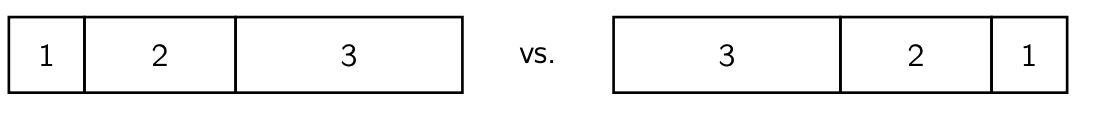
\includegraphics[scale=0.5]{scheduling_intuition.png}
\end{figure}

In the first case, assuming they all have equal weights of $1$, $\sum^{3}_{i=1} w_ic_i = 1 + 3 + 6 = 10.$ In the second case, $\sum^{3}_{i=1} w_ic_i = 3 + 5 + 6 = 14.$

\subsection{Optimal Substructure}

What do we do in the cases where $l_i < l_j$ and $w_i < w_j$? Consider the optimal ordering of jobs. Suppose we have a job $i$ that is followed by job $j$ in the optimal order. Consider swapping jobs $i$ and $j$. The example below swaps jobs 1 and 2.

Note that swapping jobs $i$ and $j$ does not alter the completion times for every other job and only changes the completion times for $i$ and $j$. $c_i$ increases by $l_j$ and $c_j$ decreases by $l_i$. This means that our objective function $\sum_i w_ic_i$ changes by $w_il_j -w_jl_i$. Since we assumed our order was optimal originally, our objective function cannot decrease after swapping the jobs. This means,
$$
w_il_j - w_jl_i \geq 0
$$
which implies
$$
\frac{l_j}{w_j} \geq \frac{l_i}{w_i}
$$

Therefore, we want to process jobs in increasing order of $\frac{l_i}{w_i}$, the ratio of the length to the weight of each job. The algorithm also does a single pass over jobs, and thus only requires $O(n)$ time, assuming the jobs were ordered by $\frac{l_i}{w_i}$. Like previously, if the algorithm also needed to sort the jobs based on the ratio of length to weight, then its runtime would be $O(n \log n)$.

\section{Optimal Codes}

Our third example comes from the field of information theory. In ASCII, there is a fixed $8$
bit code for each character. Suppose we want to incorporate information about frequencies
of characters to obtain shorter encodings. What if we want to represent characters by codes
of different lengths depending on each character's frequencies? We explore a greedy solution
to find the optimal encoding of characters.

To create optimal codes, we want a way to encode and decode our sequence. To encode the
sequence, we would just have to concatenate the code of each character together. How about
for decoding? Consider the following codes of characters: $a \to 0, b \to 1, c \to 01$. However,
when decoding, when we encounter $01$, this could be decoded as ``ab''or ``c''. Therefore, our
codes need to be prefix free: no codeword is a prefix of another.


\subsection{Tree Representation}
We may think of representing our codes in a tree structure, where the codewords represent the leaves of our tree. An example is shown below:

\begin{figure}[h!]
\centering
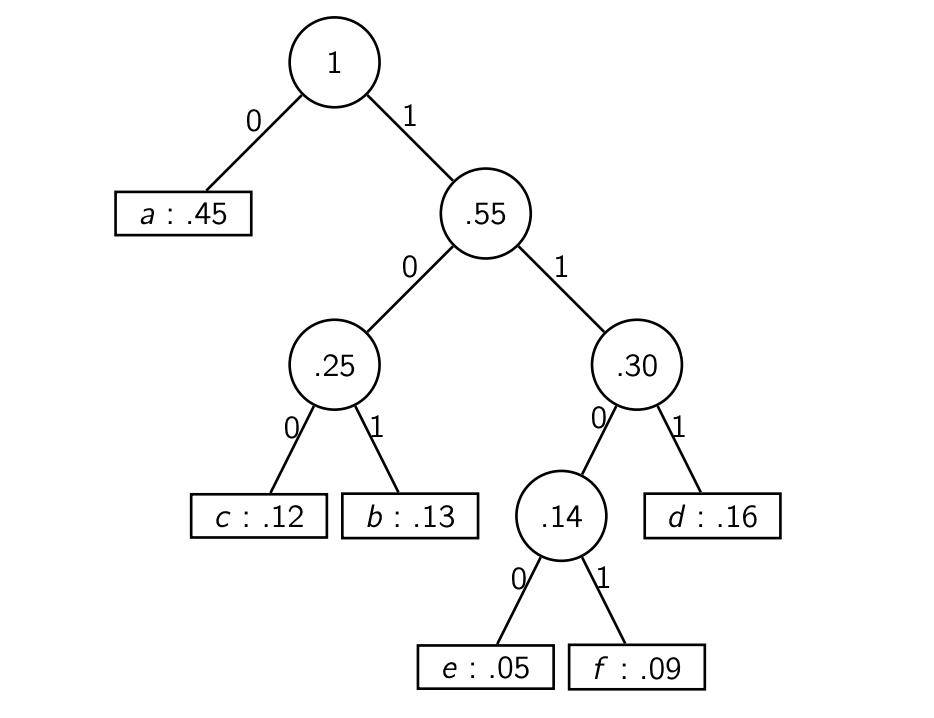
\includegraphics{huffman_tree.png}
\end{figure}
 
Above, in addition to the characters $\{a, b, c, d, e, f \}$, we've included frequency information. That is, $f (a) = 0.45$ means that the probability of a random character in this language being equal to a is $.45$. The code for each character can be found by concatenating the bits of the path from the root to the leaves. By convention, every left branch is given the bit 0 and every right branch is given the bit 1.

As long as the characters are on the leaves of this tree, the corresponding code will be 
prefixfree. This is because one string is a prefix of another if and only if the node corresponding to the first is an ancestor of the node corresponding to the second. No leaf is an ancestor of any other leaf, so the code is prefix-free.


\subsection{How good is a code?}
Suppose we have a set of characters $C$ with frequencies$ f (c)$ so that $\sum_{c\in C} f (c) = 1$. That is, $f (c)$ can be thought of as the probability of using a letter $c$ in this language. The cost, in terms of bits, of a character $c \in C$ when using the coding scheme represented by a tree $T$ is just the depth in the tree $T$: $\text{cost}(c) = d_T(c)$. For example, in the tree above, $e$ has depth 4 in the tree, and requires 4 bits to represent. The average cost of the tree is
$$
B(T) = \mathbb{E}_{c \in C}[d_t(C)] = \sum_{c \in C} f(c)d_T(c)
$$

We say that a tree $T$ is optimal if this expected cost $B(T)$ is as small as possible.

\subsection{Huffman Codes}

In 1951, David A. Huffman, in his MIT information theory class, was given the choice of a
term paper or final exam. Huffman chose to do the term paper rather than take the final
exam. He found greedy algorithm to find the most efficient binary code, which we know today
as Huffman codes.

The basic idea is this: build subtrees for subsets of characters and merge them from the
bottom up, combining the two trees with the characters of minimum total frequency.

\begin{algorithm}
\caption{A high-level description of the Huffman Coding algorithm}
\label{alg:huffman_algo}
\begin{algorithmic}
\State \textbf{Input:} Set of characters $C = \{c_1, c_2, \cdots, c_n \}$ of size $n$, and $F = \{f(c_1), f(c_2), \cdots, f(c_n) \}$, a set of frequencies.
\State Create nodes $N_k$ for each character $c_k$ with key $f(c_k)$
\State Let the \texttt{current} denote the set $\{N_1, \cdots, N_n\}$ of nodes.
\State \While {\texttt{current} has \textit{length of more than one}} {
    \State Find the two nodes $N_i$ and $N_j$ in the \texttt{current} with the minimum frequencies and create a new intermediate node $I$ with $N_i$ and $N_j$ as its children, so that $I$.key $= N_i$.key $+ N_j$.key.
    \State Add $I$ to the \texttt{current} and remove $N_i, N_j$
}
\State \Return \textit{the only entry of \texttt{current}, which is the root of the tree}
\end{algorithmic}
\end{algorithm}

The tree shown above results from running this algorithm on the letters with those frequencies; see the slides for an illustration of this process.

\subsection{Proof of Correctness}

This algorithm works, but at first it's not at all obvious why. For a rigorous proof, refer to
Lemmas 16.2 and 16.3 in CLRS. However, we'll sketch the idea below. Formally, the proof
goes by induction. Recall that after iteration t in Algorithm \ref{alg:huffman_algo}, we have a list current, which contains the roots of subtrees that we still need to merge up. We will maintain the following inductive hypothesis:

\begin{itemize}
    \item \textbf{Inductive hypothesis}: Suppose we have completed $t$ iterations of the loop in Algorithm \ref{alg:huffman_algo}. Then there exists a way to merge the subtrees in current that is optimal.
    \item For the \textbf{base case}, we observe that when $t = 0$, current is just the set of all characters, and definitionally there exists an optimal tree made out of these nodes.
    \item For the \textbf{inductive step}, we need to show that if the inductive hypothesis holds at step $t - 1$, then it holds at step $t$. We'll sketch this later.
    \item Finally, to conclude the argument, we see that at the end of the algorithm, there is only one element in current, and in this case the inductive hypothesis reads that there is a way to merge this single subtree to obtain an optimal subtree. That's just a convoluted way of saying that the single tree we return is optimal, and so we are done.
\end{itemize}
All that remains to show is the inductive step. We first observe the following claim:

\begin{proposition}
We are given a set of characters $C$ and a set of its associated frequencies $F$ where $f (c)$ is the frequency of character $c$. Let $x$ and $y$ be the characters with the two smallest frequencies. There exists an optimal coding tree for $C$ such that $x$, $y$ are sibling leaves.
\end{proposition}

\begin{proof}
Let $T$ be the optimal coding tree for $C$. The optimal coding tree must be a full binary
tree, that is, every non-leaf node must have two children. Let a, b be characters that are
sibling leaves of maximum depth. We define the number of bits to encode $c$ as $d_T (c)$ and
the number of bits needed for the coding tree as $B(T) = \sum_c f(c)d_T(c)$.

We can replace $a, b$ by $x, y$ without increasing the total number of bits needed for the coding
tree.\footnote{For simplicity, we ignore the case where $a, b, x, y$ are not distinct. For more details, see Lemma 16.2 in CLRS} If we swap $x$ and $a$, the change in cost becomes $f (x)d_T (a) + f (a)d_T (x) - f (x)d_T (x) - f (a)d_T (a) = (f (x) - f (a))(d_T (a) - d_T (x)) \leq 0$

Therefore, swapping $a, b$ with $x, y$ will not increase our objective function $B(T)$. Hence, there exists an optimal coding tree where x, y are siblings in the tree.
\end{proof}

\begin{proposition} 
Let $C$ be a set of characters, and let $T$ be an optimal coding tree for $C$. Imagine creating $C'$ from $C$ by collapsing all the characters in a subtree rooted at a node $N$ with key $k = N$.key into a single character $c'$ with frequency $k$. Then the corresponding tree $T'$ is optimal for $C'$ . Conversely, suppose that a tree $T'$ that is an optimal coding tree for an alphabet $C'$ . Let $c'\in C'$ be a character with frequency $f (c')$. Introduce new characters $c_1'' , \cdots , c_r''$ with total frequency $\sum^{r}_{i=1} f (c''i ) = f (c')$. Let $T'$ be an optimal coding tree on $c''_1 , \cdots , c''_r$ . Then the tree $T$ on the alphabet $C = (C'\setminus \{c'\}) \cup \{c''_1 , \cdots , c''r \}$ that has the leaf $c'$ replaced with the subtree $T'$ is optimal.
\end{proposition}


\begin{proof}
Let T and T' be the two trees described in the lemma, and consider the difference of their costs.

\begin{align*}
B(T) - B(T') &= \sum_{c\in C} f(c) \cdot d_T(c) - \sum_{c \in C'} f(c) d_{T'}(c) \\
&= \left(\sum_{i=1}^r f(c_i'' d_T(c_i'')) - f(c')d_{T'}(c') \right) \\
&= \left(\sum_{i=1}^r f(c_i'')(d_{T''}(c_i'') + d_{T'}(c'))\right) - f(c')d_{T'}(c') \\
&= \sum_{i=1}^{r} f(c_i'')d_{T''}(c_i'') + d_{T'}(c')\sum_{i=1}^r f(c_i'') - f(c')d_{T'}(c') \\
&= \sum_{i=1}^t f(c_i'')d_{T''}(c_i'')
\end{align*} 

where the last line used the fact that $\sum^{r}_{i=1} f (c ''_i ) = f (c ' )$, and so the last two terms cancelled. This means that the difference in the cost between these two trees only depends on $T''$, it doesn't depend at all about the structure of $T$. Thus, $T$ is optimal if and only if $T'$ is optimal.
\end{proof}

The two Claims together prove the inductive step, because the second claim implies that the logic of the first claim holds, even for newly created intermediate nodes $I$.

\textbf{Note}: The proof in CLRS has the same basic steps (Lemmas 16.2 and 16.3 instead of the claims above), although phrased slightly differently. The sketch above is pretty sketchy, so if the above is hard to follow, please check out CLRS for a more detailed version.



























\end{document}
